\documentclass{article}
\usepackage{fullpage}
\usepackage[utf8]{inputenc}
\usepackage{graphicx}
\usepackage[ngerman]{babel}
\usepackage{hyperref}
\usepackage{tabularx}
\usepackage{attachfile}
\usepackage{pdfpages}
\usepackage{siunitx}
\usepackage{caption} \captionsetup[table]{skip=10pt}
\usepackage[demo]{graphicx}
\usepackage{subfig}
\usepackage{float}

\title{Ausarbeitung zu Schiefe Ebene (SEB)}
\author{Anfängerpraktikum Teil 1 \\Technische Universität München\\\\Leon Heiß, Paul Hildebrandt \\
Kurs 5, Gruppe 7, Team 19}
\date{21. Juni 2022}
\renewcommand*\contentsname{Inhaltsverzeichnis}

\renewcommand{\abstract}[1]{{ \noident {\bf\\Einleitung \\} #1 }}

\begin{document}

\maketitle

\large
\begin{center}
\textbf{Abstract}\\
\normalsize
\medskip
In diesem Versuch werden die Kräfte näher untersucht, die auf einen Körper wirken, der sich auf einer schiefen Ebene befindet. Dabei liegt der Fokus auf der Kräftezerlegung sowie der Bestimmung des Haftreibungs- bzw. des Gleitreibungskoeffizienten.

\end{center}
\normalsize

\tableofcontents

\section{Grundlagen}
\subsection{Kräftezerlegung}
Betrachtet man einen beliebigen Körper, der sich auf einer Ebene befindet, kann man die auf ihn wirkende Gewichtskraft $F_G$ in zwei Komponenten aufteilen, nämlich eine Komponente $F_{\bot}$ senkrecht und eine Kraft $F_{\parallel}$ parallel zur Ebene.
\begin{figure}[hbt!]
\centering
\includegraphics[width=200pt]{zerlegung.png}
\caption{Kräftezerlegung an der schiefen Ebene \cite{1}.}
\label{fig:length_eight_mouse}
\end{figure}
Beschreibt man wie in Abbildung 1, den Neigungswinkel der Ebene zur Oberfläche mit $\alpha$, erhält man für die beiden Komponenten der Gewichtskraft:
\begin{equation}
    F_{\bot} = F_g \cdot \cos(\alpha) = mg \cos \alpha
\end{equation}
\begin{equation}
    F_{\parallel} = F_g \cdot \sin(\alpha) = mg \sin \alpha.
\end{equation}
\subsection{Gleit- und Haftreibung}
An der Grenzfläche zwischen der Ebene und dem Körper treten Reibungskräfte parallel zur der Fläche auf. Man unterscheidet zwischen Gleitreibung und Haftreibung. Solange die beschleunigende Kraft kleiner als die Haftreibungskraft $F_H$ ist, bleibt der Körper in Ruhe. Wird die Haftreibungskraft überwunden, beginnt der Körper sich zu bewegen und die Gleitreibungskraft $F_R$ wirkt entgegen der Bewegungsrichtung, welche abhängig von der Normalkomponente $F_{\bot}$ der Gewichtskraft und dem Gleitreibungskoeffizienten $\mu_G$ ist:
\begin{equation}
    F_R = \mu_G \cdot F_{\bot}.
\end{equation} Die Haftreibungskraft lässt sich analog mit dem Haftreibungskoeffizienten $\mu_H$ bestimmen:
\begin{equation}
    F_H = \mu_H \cdot F_{\parallel}.
\end{equation}
Die beiden Reibungskoeffizienten sind materialabhängige Konstanten, wobei die Gleitreibung immer
kleiner als die Haftreibung sein muss. Auf der schiefen Ebene erhält man die beschleunigende Kraft $F_a$ auf einen Körper mit der Masse $m$ durch die Differenz aus der angreifenden Kraft und der Reibungskraft:
\begin{equation}
    F_a = m \cdot a = F_{\parallel} - \mu \cdot F_{\bot} = F_g \cdot (\sin \alpha - \mu \cos \alpha),
\end{equation} solange $\sin \alpha \geq \cos \alpha$. Die Konstante $\mu$ bezeichnet hierbei entweder $\mu_G$ oder $\mu_H$. Wenn die angreifende Kraft nun der  Haftreibungskraft entspricht, der Körper also gerade noch nicht rutscht, gilt:
\begin{equation}
    \mu_H= \tan \alpha.
\end{equation}
\section{Überprüfen der Kräftezerlegung}
\subsection{Versuchsaufbau}
In diesem Teilversuch betrachtet man einen Rutscher (Abbildung 2a), auf den bis zu drei Gewichte
aufgesteckt werden können, welcher sich auf einer Ebene mit variablem Neigungswinkel $\alpha$ befindet. Zudem können Kraftmesser angebracht werden, sodass die tangentiale und die normale Kraft auf den Rutscher gemessen werden können (Abbildung 2b). Nun bring man die beiden Kraftmesser an und zieht an dem normalen Kraftmesser, bis der Rutscher geradeso über der Ebene schwebt. An dieser Stelle wird nun Normal- und Tangentialkraft abgelesen. Der Versuch wird dann für verschiedene Winkel $\alpha$ durchgeführt.
\begin{figure}
    \centering
    \subfloat[\centering Aufbau des Rutschers \cite{1}]{{\includegraphics[width=7cm]{rutscher1.png} }}%
    \qquad
    \subfloat[\centering Versuchsaufbau zur Überprüfung der Kräftezerlegung \cite{1}]{{\includegraphics[width=7cm]{rutscher2.png} }}%
    \caption{}
    \label{fig:example}%
\end{figure}
\subsection{Auswertung}
Betrachtet man Gleichung 1 und 2, erkennt man, dass für den
vom Neigungswinkel abhängigen Quotienten von Tangential- zu Gewichtskraft $\frac{F_{\parallel}}{F_{g}} = \sin \alpha$ gilt. Analog erwartet man auch, dass $\frac{F_{\bot}}{F_{g}} = \cos \alpha$ und $\frac{F_{\parallel}}{F_{\bot}} = \tan \alpha$ gilt. Die Verhältnisse sind jeweils mit den Theoriefunktionen in Abbildung 3,4 und 5 aufgetragen.
Man erkennt, dass die Werte der Quotienten zwar in den richtigen Größenordnungen liegen, es aber doch merkliche Abweichungen zu den theoretischen Werten gibt. Innerhalb der Unsicherheiten kann man hier aber schon von einer erfolgreichen Näherung sprechen.
\begin{figure}[hbt!]
\centering
\includegraphics[width=470pt]{zerplot1.png}
\caption{Verhältnis von Tangentialkraft zu Gewichtskraft.}
\label{fig:length_eight_mouse}
\end{figure}
\begin{figure}[hbt!]
\centering
\includegraphics[width=470pt]{zerplot2.png}
\caption{Verhältnis von Normalkraft zu Gewichtskraft.}
\label{fig:length_eight_mouse}
\end{figure}
\begin{figure}[hbt!]
\centering
\includegraphics[width=470pt]{zerplot3.png}
\caption{Verhältnis von Tangentialkraft zu Normalkraft.}
\label{fig:length_eight_mouse}
\end{figure}
\subsection{Fehlerrechnung}
In diesem Teilversuch sind zwei Unsicherheiten zu beachten. Zunächst wäre da die Ablesegenauigkeit der jeweiligen Kraftmessern, welche berücksichtigt werden müssen. Diese belaufen sich von $0.02$ bis $0.1$ für die stärkste Feder. Des Weiteren besteht eine Ungenauigkeit bei der Bestimmmung des Winkels. Wir entschieden uns die Neigung der schiefe Ebene mittels des eingebauten Gyroskops eines Smartphones zu bestimmen, welches wir mit einer Ungenauigkeit von 0,5$\deg$ notierten.
\section{Bestimmung des Haftreibungskoeffizienten}
\subsection{Versuchsaufbau}
Der Haftreibungskoeffizient kann bestimmt werden, indem man den Rutscher auf eine waagrechte Ebene
platziert und an dem tangentialen Kraftmesser zieht, bis sich der Rutscher gerade bewegt, die
Haftreibungskraft also geradeso überwunden wird. Es wird nun die gemessene Kraft notiert, bei der sich der Rutscher bewegt hatte. Die Messung wird dann für den Rutscher mit ein und zwei Gewichtscheiben wiederholt und jeweils 20 mal durchgeführt.
\subsection{Auswertung}
Um die mittlere Haftkraft zu ermitteln, muss lediglich der Mittelwert aus allen Messwerten gebildet werden, da die Kraft, bei der sich der Rutscher gerade zu bewegen beginnt, betragsmäßig gleich groß wie die Haftkraft ist. Zeichnet man diese gegen die unterschiedlichen verwendeten Massen auf, ergibt sich folgender Graph:
\begin{figure}[hbt!]
\centering
\includegraphics[width=470pt]{haftreibungsfit.png}
\caption{Mittlere Haftreibungskraft aufgetragen gegen Masse mit Unsicherheiten.}
\label{fig:length_eight_mouse}
\end{figure}
Die eingetragene Ausgleichsgerade (Abbildung 6) geht nicht, wie zu erwarten wäre, genau durch den Ursprung, was wahrscheinlich an Messunsicherheiten bei der Kraftmessung liegt.
Nun kann der Haftreibungskoeffizient bestimmt werden, indem man Gleichung 4 nach $\mu_H$ umstellt und für $F_{\bot}$ die Gewichtskraft $F_g = m \cdot g$ des jeweiligen Rutschers einsetzt. Mit der zuvor berechneten mittleren Haftreibungskraft $F_H$ ergeben sich somit folgende Werte:

\begin{table}[H]
\caption{Haftreibungskoeffizienten}
\centering
\begin{tabular}{| >{\centering\arraybackslash}m{5cm} | >{\centering\arraybackslash}m{5cm} | >{\centering\arraybackslash}m{5cm} |}
\hline
\rule{0pt}{10pt}
verwendete Masse m [g] & mittlere Haftkraft $F_H$ [N] & Haftreibungskoeffizient $\mu_H$ \\ \hline
 284,40 $\pm$ 1 & 1 $\pm$ 0,117 & 0,3585 $\pm$ 0,042 \\ \hline
 867,92  $\pm$ 1 & 3,51 $\pm$ 0.334 & 0,4124 $\pm$ 0,039\\ \hline
 1451,44 $\pm$ 1 & 6,66 $\pm$ 0,539 & 0,4679 $\pm$ 0,038 \\ \hline
\end{tabular}
\end{table}
\subsection{Fehlerrechnung}
In diesem Teilversuch müssen zwei wichtige Unsicherheiten beachtet werden. Zunächst berücksichtigt man die Typ-A-Unsicherheit des Kräftemessens, indem man die Standartabweichung des Mittelwerts der 20 Messungen bestimmt:
\begin{equation}
   \sigma_{\bar{x}} = \frac{1}{\sqrt{n}} \cdot \sqrt{\frac{1}{n-1} \cdot \sum^n_{i=1}} (x_i \cdot \bar{x})^2 .
\end{equation} Des Weiteren liegen bei der Messung Typ-B-Unsicherheiten durch die Ablesegenauigkeit der Kraftmesser vor, da diese aber deutlich kleiner als die Standartabweichung sind, kann man sie vernachlässigen. Die Unsicherheit für die Masse wurde in diesem Teilversuch auf $u(m) = \pm  1$g geschätzt, da das Gewicht des Rutschers mit verschiedenen Kraftmessern gemessen wurde, welche alle eine unterschiedliche Ablesegenauigkeit besitzen, die nicht notiert wurde.
Die Unsicherheit des Haftreibungskoeffizienten $u(\mu_H)$ lässt sich nun mithilfe der Gaußschen Fehlerfortpflanzung bestimmen:
\begin{equation}
    u(\mu_{H}) = \sqrt{\bigg(\frac{u(F_H)}{F_G}\bigg)^2+\bigg(\frac{F_H \cdot u(F_G)}{F_G^2}\bigg)^2}.
\end{equation}
\section{Bestimmung des Gleitreibungskoeffizienten}
\subsection{Versuchaufbau}
Um den Gleitreibungskoeffizienten zu bestimmen müssen die Kräfte am Gleiter betrachtet werden, während er in Bewegung ist.
Der Koeffizient bestimmt, mit welcher Beschleunigung sich der Gleiter die schiefe Ebene hinunter bewegt.
Um die Beschleunigungen möglichst genau zu dokumentieren, wird ein Ultraschallsensor mit einer Abtastrate von 25Hz verwendet.
Für jeden Winkel der schiefen Ebene werden mindestens drei Messungen durchgeführt.
Die Winkel werden jeweils mittels Beschleunigungssensor eines Smartphones dokumentiert.
Bei niedrigem Winkel wird ein Gleiter mit größerem Gewicht verwendet, um Unebenheiten auf der Oberfläche durch die höhere Trägheit zu kompensieren.
Bei höherem Winkel ein kleineres Gewicht, da das schnelle Abbremsen des Gleiters von Hand sonst nur schwer möglich ist.
Das Gewicht hat in einem idealen System keine Auswirkung auf die Beschleunigung.
\subsection{Auswertung}
Zunächst werden die Positionskurven mit einem Polynom zweiten Grades gefittet.
\begin{figure}[hbt!]
\centering
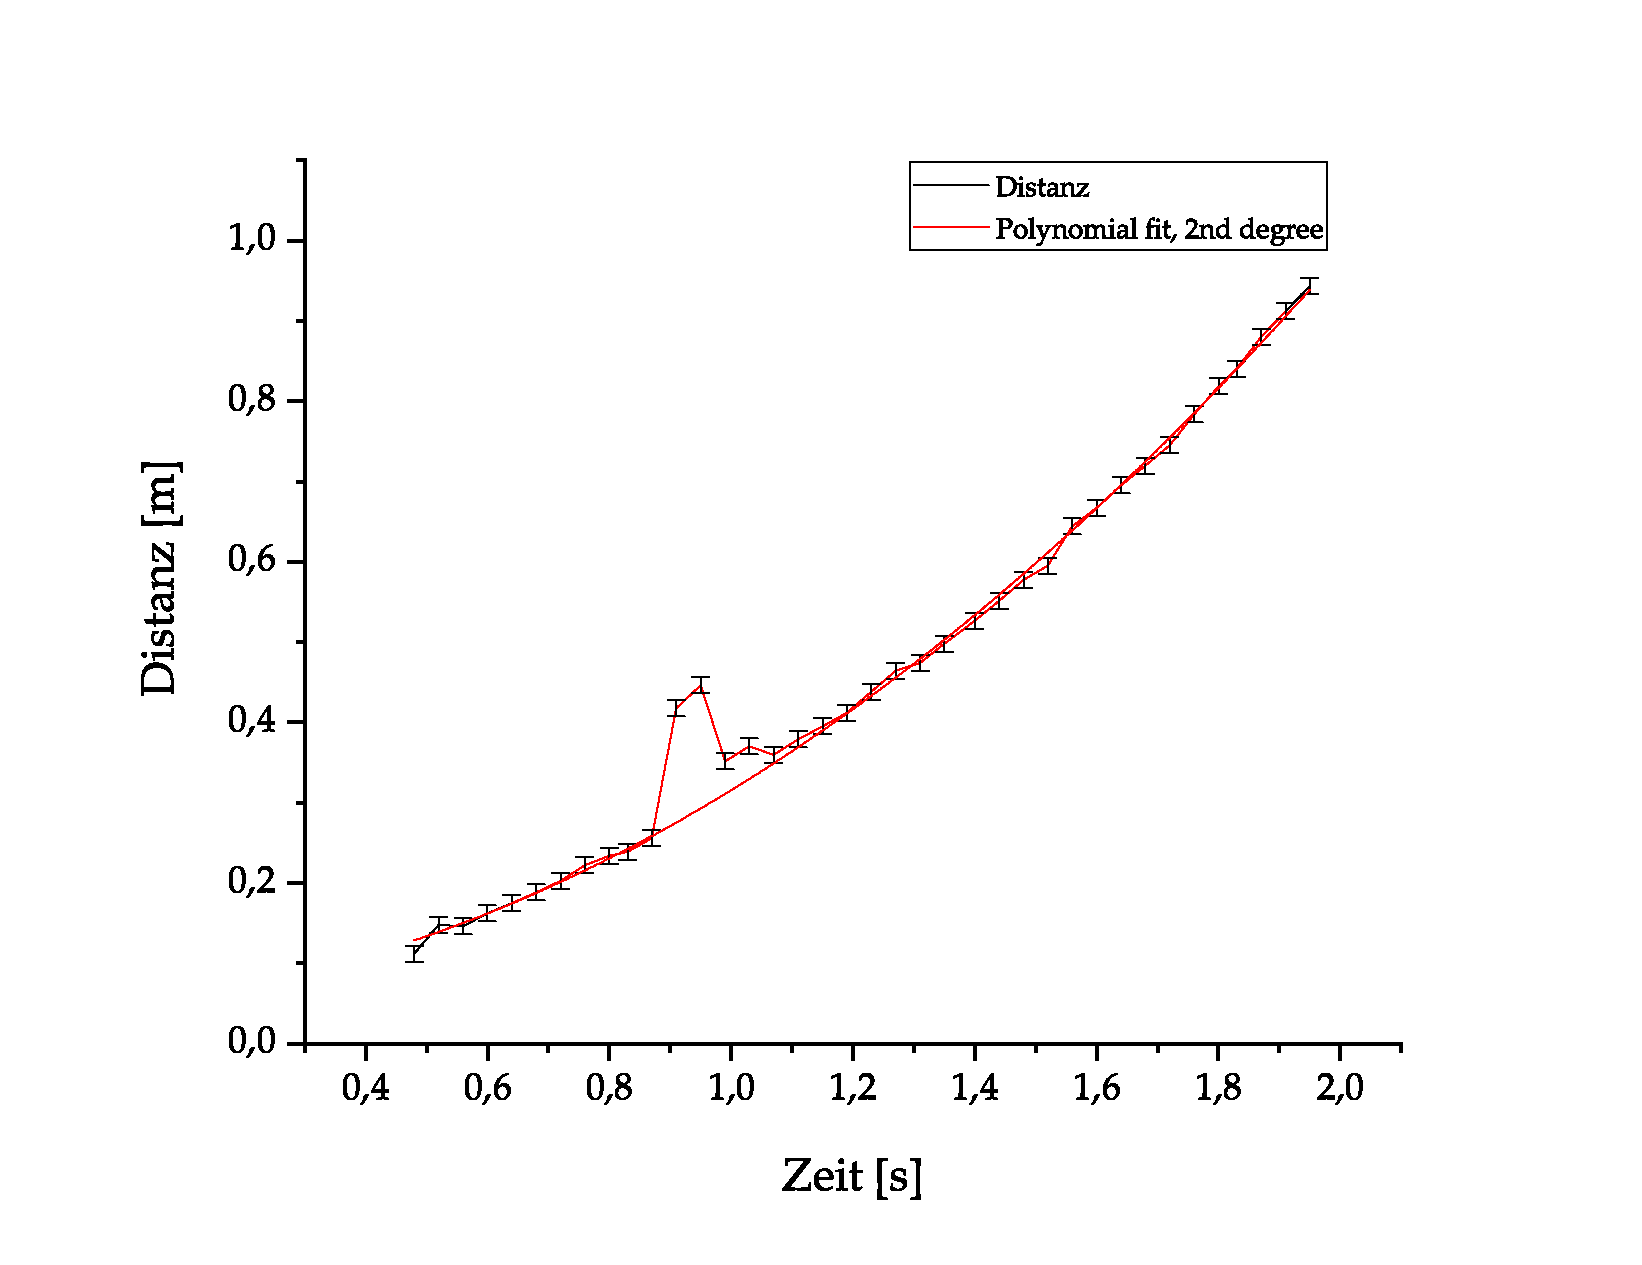
\includegraphics[width=300pt]{PolynomFit.eps}
\caption{Fit von Positionsdaten mit einem Polynom zweiten Grades.}
\end{figure}
Da wir nur an der Beschleunigung interessiert sind, die der zweiten Ableitung des Ortes entspricht, erhalten wir durch zweifaches Ableiten des Polynoms einen Beschleunigungswert.
Die verschiedenen erhaltenen Werte für jede Versuchskonfiguration werden mit Hilfe des gewichteten Mittelwertes zusammengefasst.
Man erhält einen Beschleunigungswert für jede Steigung:
\begin{center}
\begin{tabular}{|c|c|}
\hline 
Winkel [$\deg$] & Beschleunigung [m/s$^2$] \\ 
\hline 
18,10(0,5) & 0,3609(0,0169) \\ 
\hline 
26,10(0,5) & 1,9612(0,1737) \\ 
\hline 
34,50(0,5) & 2,4640(0,1479) \\ 
\hline 
44,65(0,5) & 4,1741(0,1779) \\ 
\hline 
\end{tabular} 
\end{center}
Die auf den Gleiter in Bewegungsrichtung wirkenden Kräfte lassen sich beschreiben mit
\begin{equation}
F_{ges,tan} = F_{g,tan}+F_R = sin(\theta)\cdot m \cdot g - cos(\theta) \cdot m \cdot g \cdot k
\end{equation}
mit dem Gleitreibungskoeffizienten $k$.
Die resultierende Beschleunigung ist gegeben durch
\begin{equation}
a_{ges,tan} = sin(\theta) \cdot g - cos(\theta) \cdot g \cdot k.
\end{equation}
Dies lässt sich umformen zu
\begin{equation}
\frac{a_{ges,tan}}{g} = sin(\theta) - k \cdot cos(\theta). 
\end{equation}
Alle Werte außer $k$ sind bekannt. $k$ lässt sich demnach berechnen. Da wir allerdings mehrere Werte zu einem $k$ zusammenfassen wollen, versuchen wir, k aus einem Fit der genannten Theoriefunktion zu bestimmen.
Hierzu wird $ratio = \frac{a_{ges,tan}}{g}$ gegen den Winkel $\theta$ aufgetragen.
\begin{figure}[H]
\centering
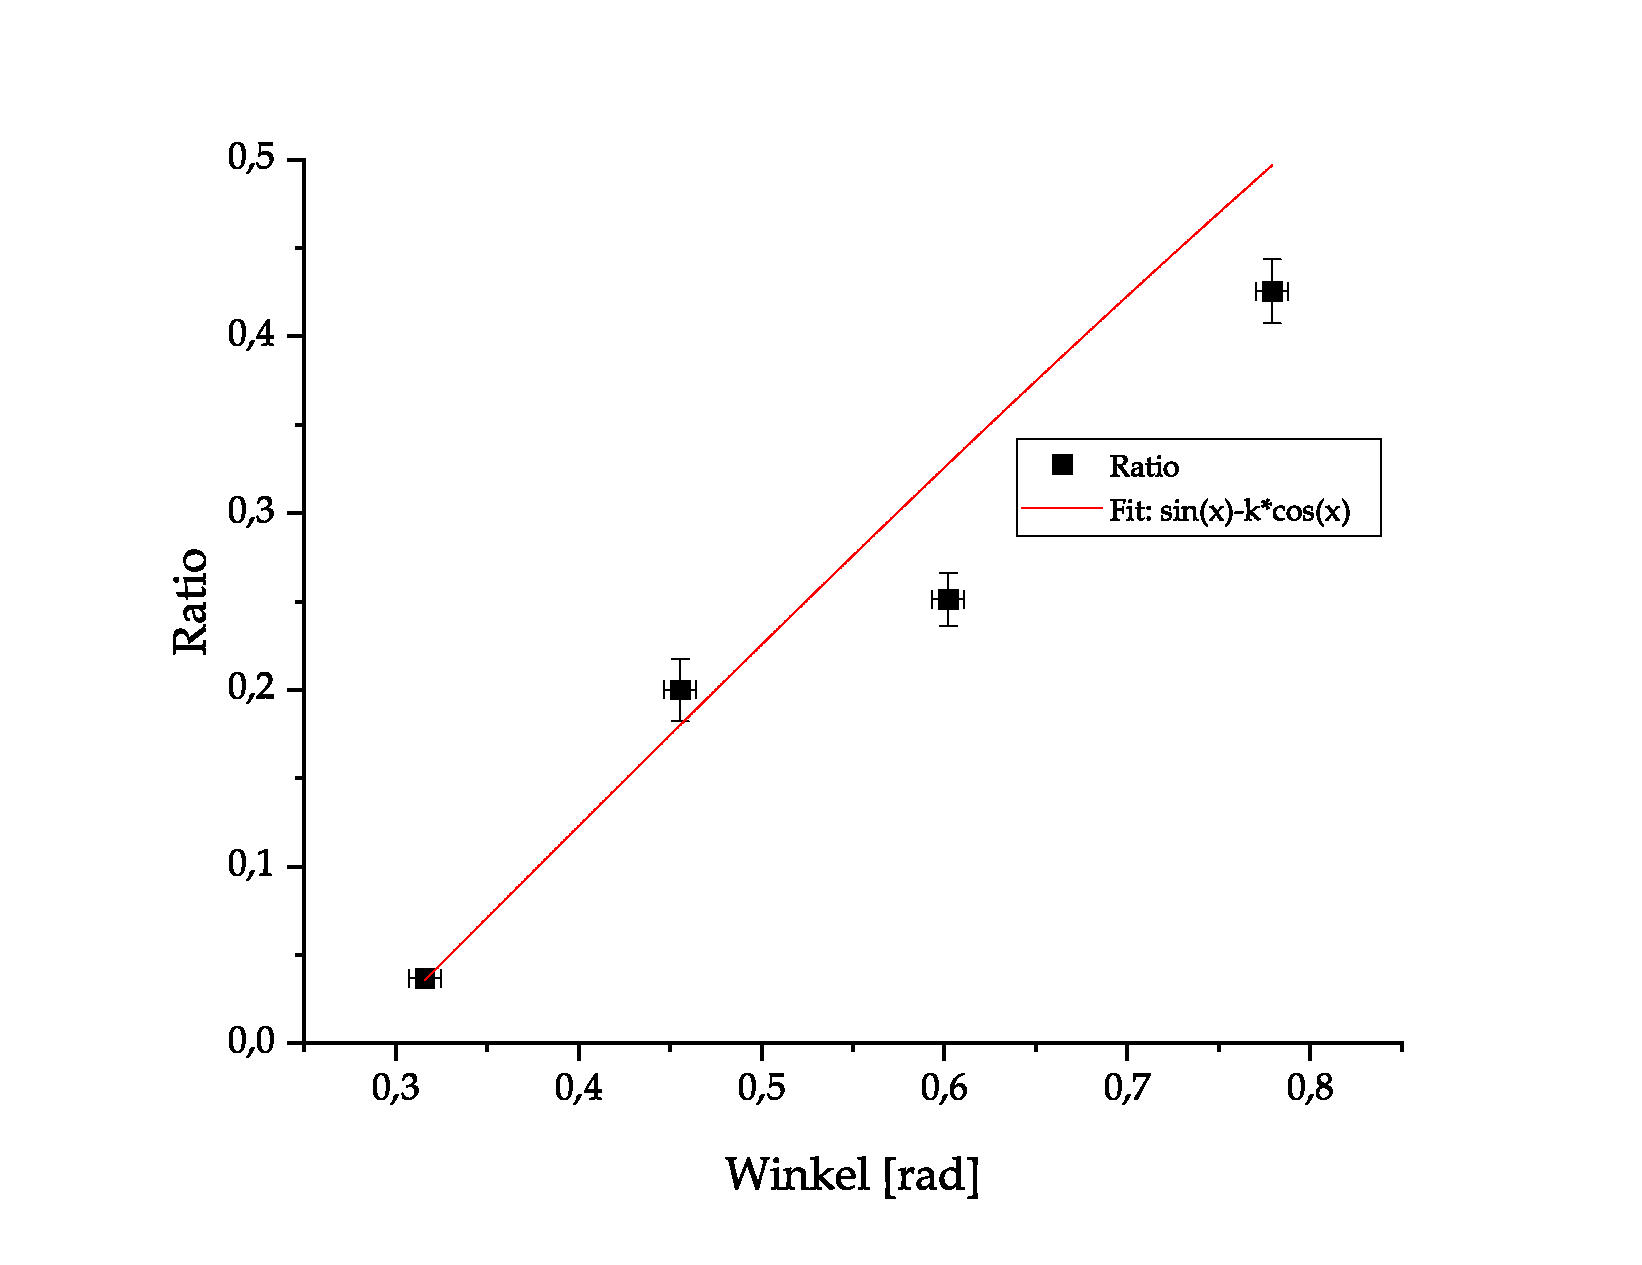
\includegraphics[width=300pt]{FitGleitreibung.eps}
\caption{Fit der verschiedenen Beschleunigungsverhältnisse zur Bestimmung des Gleitreibungskoeffizienten}
\end{figure}
Man erhält einen Wert von $k = 0,289(0,007)$.
Dieser Wert scheint realistisch und stimmt mit dem Literaturwert $\cite{2}$ überein.
\subsection{Fehlerrechnung}
Eingangsfehler sind die Distanzmessung und der Winkel der Ebene. Für die Distanz wird eine Varianz von 1cm angenommen. Diese wird in den Fit des Polynoms zweiten Grades mit einbezogen. Die Ergebnisse des gewichteten Mittelwertes erhalten ihre Unsicherheit gemäß der im ABW-Skript in Formel 29 bis 32 \cite{3} gegebenen Berechnungsmethode . Es resultieren die oben genannten Beschleunigungswerte und ihre Unsicherheiten. Für den letzten Fit muss nun ebenfalls die Varianz des Winkels einbezogen werden, welche wir wie zuvor auf 0,5$\deg$ geschätzt haben.
\section{Literaturverzeichnis}
\begin{thebibliography}{9}
\bibitem{1}
Fakultät für Physik. \emph{Schiefe Ebene} (SEB. Technische Universität München. 24.06.2022.
\textbf{URL:} \url{https://www.ph.tum.de/academics/org/labs/ap/ap1/AKU.pdf}

\bibitem{2}
schweizer-fn \emph{Formelsammlung und Berechnungsprogramme Maschinen- und Anlagenbau} (Gleitreibwerte von verschiedenen Materialien. 24.06.2022.
\textbf{URL:} \url{https://www.schweizer-fn.de/stoff/reibwerte/reibwerte_gleitreibung.php#holz}

\bibitem{3}
Fakultät für Physik. \emph{ABW-Skript} (24.06.2022).
\textbf{URL:} \url{https://www.ph.tum.de/academics/org/labs/ap/org/ABW.pdf}

\end{thebibliography}
\section{Anhang}
\subsection{Laborbuch}
\includepdf[pages=-]{Protokoll.pdf}
\end{document}
